\begin{figure}[h]
  
\includegraphics[scale=0.3]{images/they-work-for-you-challenges-finance}
  \caption{They Work for You: banner advert for donations}
  \label{fig:they-work-for-you-challenges-finance}
\end{figure}

A second challenge facing They Work for You, and one that they may well share with many charitable orhganisations, is a lack of finance.
To that end, Figure \ref{fig:they-work-for-you-challenges-finance} depicts the home page of the site with an apparently permanent banner advert for donations.
That being said, and according to a Guardian article in 2008 \cite{guardian-tom-steinberg} They Work For you via parent organisation MySociety undertook paid work for the government to produce the UK e-petition site.

\begin{figure}[h]
  \centering
  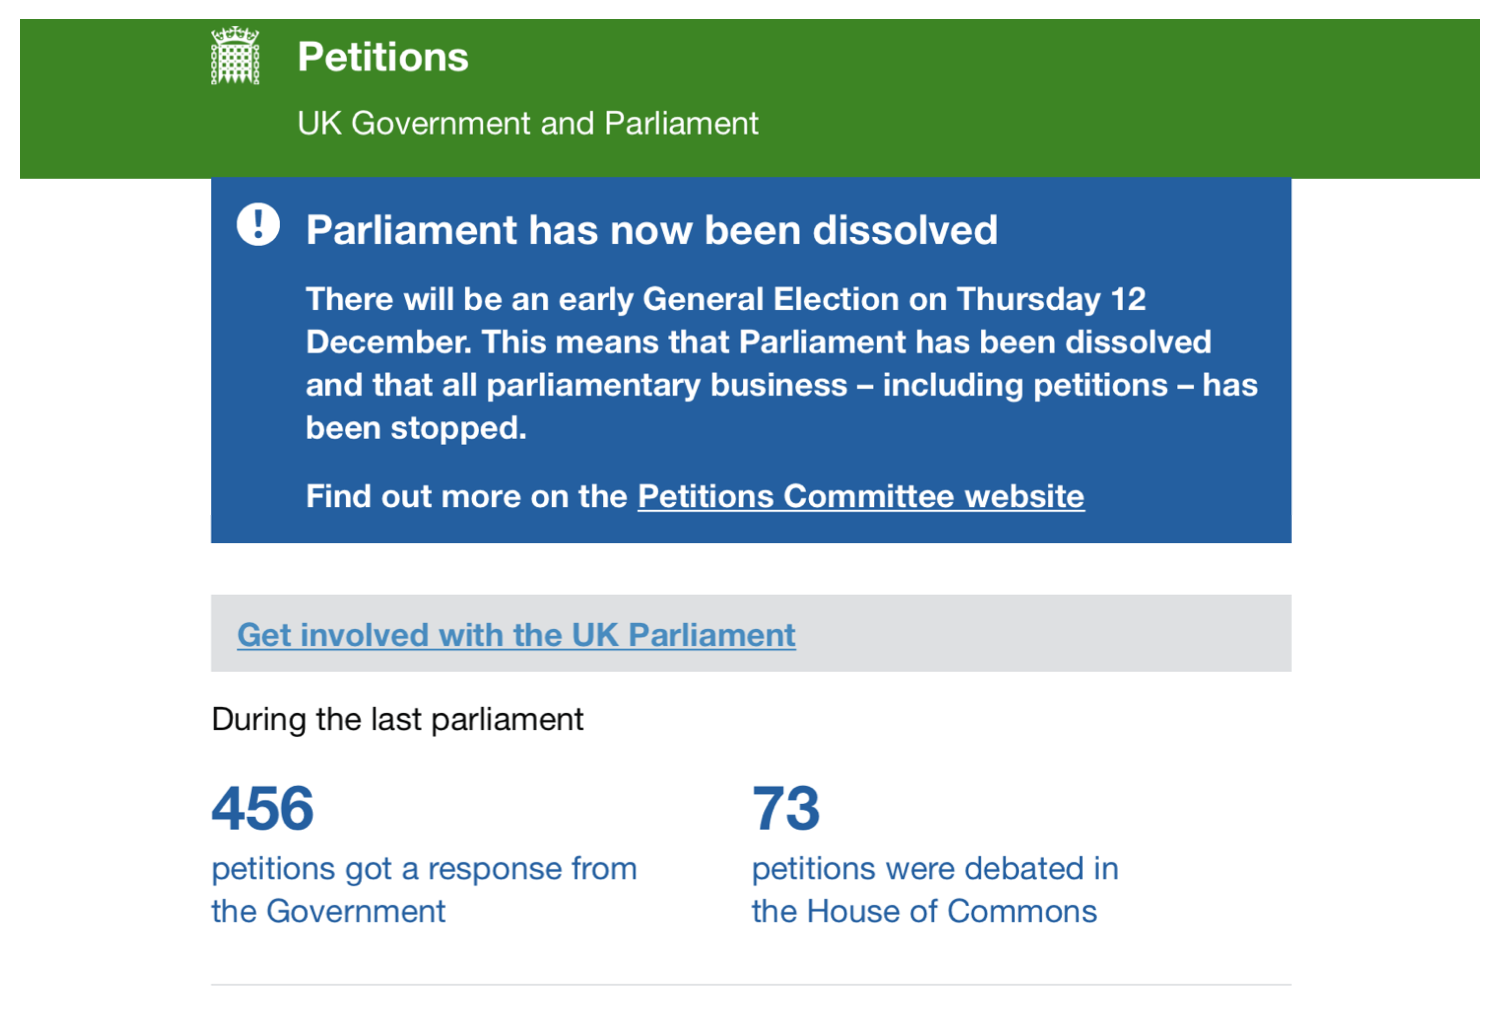
\includegraphics[scale=0.3]{images/e-petition-site}
  \caption{UK Government: E-Petition web site}
  \label{fig:e-petition-site}
\end{figure}

A screen shot of the e-petition site can be found within Figure \ref{fig:e-petition-site}.
In addition, the They Work for You now offer a paid for Application Programming Interface (or API) enabling secondary groups of individuals to access data (once an appropriate licence) has been bought.